\chapter{Planificación y cumplimiento}

\section{Diagrama de Gantt}

El diagrama de Gantt del anteproyecto organizaba el trabajo en una etapa de investigación, dos iteraciones de desarrollo, entregas intermedias, pruebas intensivas, documentación y un período final para extras. La primera iteración concentraba el pipeline, la configuración de la Raspberry Pi, el hardware base, el control físico y la integración inicial. La segunda contemplaba los ajustes de la primera versión y, si el tiempo lo permitía, la mejora y el entrenamiento de modelos.

\begin{figure}[H]
    \centering
    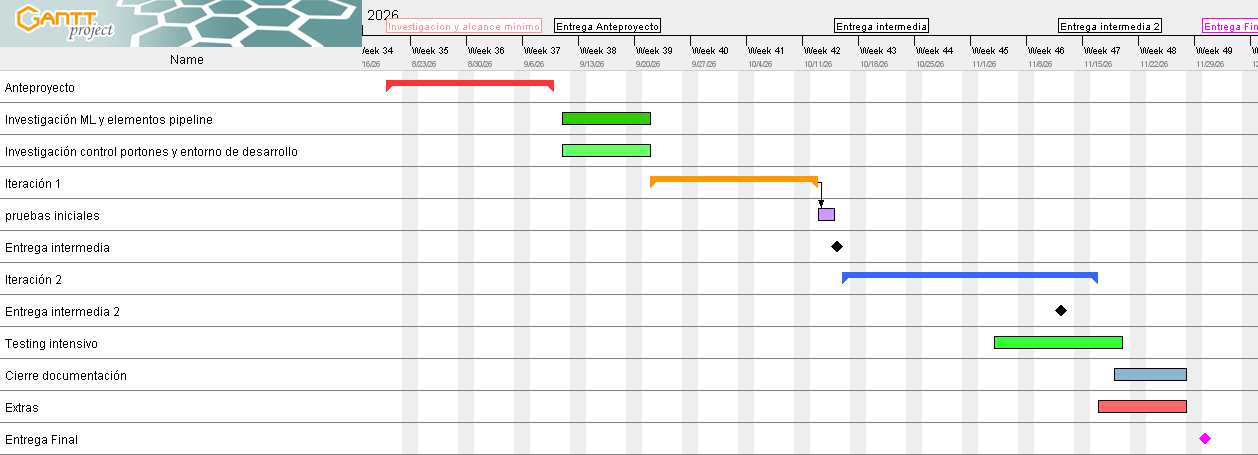
\includegraphics[width=\textwidth]{Imagenes/gantt_anteproyecto.png}
    \caption{Diagrama de Gantt del anteproyecto.}
    \label{fig:gantt}
\end{figure}

Al comparar el desarrollo realizado con el diagrama de Gantt definido al comienzo del proyecto, la planificación general pudo respetarse en buena medida. Las etapas de investigación, desarrollo de los prototipos, integración, pruebas y cierre de documentación se mantuvieron aproximadamente dentro de los períodos previstos, aunque algunas actividades debieron ejecutarse en paralelo o modificarse en función de los resultados obtenidos durante el desarrollo.

\section{Comparación con lo planificado}

La tabla~\ref{tab:cumplimiento-gantt} compara cada etapa planificada con el resultado obtenido.

\begin{table}[H]
    \centering
    \small
    \renewcommand{\baselinestretch}{1.15}\selectfont
    \begin{tabular}{|p{3.5cm}|p{2.4cm}|p{7.9cm}|}
        \hline
        \textbf{Etapa planificada} & \textbf{Resultado} & \textbf{Observaciones} \\ \hline
        Investigación y anteproyecto & Cumplida & Se definieron el alcance, la arquitectura, la plataforma y los modelos iniciales. \\ \hline
        Iteración 1 e integración del MVP & Cumplida & Se desarrollaron el pipeline, la Raspberry Pi, el control físico y las pruebas iniciales. \\ \hline
        Ajustes de la segunda iteración & Cumplida & Se modularizó el programa y se mejoró la sincronización, el manejo de estados y la recuperación ante errores. \\ \hline
        Extras operativos & Cumplida & Se implementaron Supabase, interfaz web, caché offline, eventos pendientes y systemd. \\ \hline
        Construcción del dataset & Cumplida parcialmente & Se desarrolló la herramienta de captura y se tomaron muestras, pero no se alcanzó el volumen mínimo necesario. \\ \hline
        Entrenamiento específico & No culminada & El proceso comenzó, pero la falta de datos suficientes y de tiempo impidió entrenar y validar modelos propios. \\ \hline
        Pruebas y documentación & Cumplida & Se probaron el pipeline, la cámara, el GPIO, la base de datos y el modo offline, y se consolidó el informe. \\ \hline
    \end{tabular}
    \caption{Comparación entre la planificación del Gantt y el resultado final.}
    \label{tab:cumplimiento-gantt}
\end{table}

\section{Desvíos respecto de la planificación}

\subsection{Base de datos e interfaz web en paralelo}

Una de las principales diferencias respecto a la planificación fue la incorporación de la base de datos y de la interfaz web de administración. Estas funcionalidades habían sido planteadas inicialmente como prestaciones adicionales posteriores al cumplimiento del MVP; sin embargo, se decidió avanzar sobre ellas en paralelo al desarrollo principal. Esto permitió integrar Supabase con el sistema y disponer de una gestión más completa de usuarios y registros sin desplazar como prioridad el funcionamiento del pipeline y del control de acceso.

\subsection{Entrenamiento propio no realizado}

El desvío principal respecto a lo planificado se concentró en el entrenamiento propio. No se llegó a realizar el entrenamiento o ajuste específico de los modelos con un dataset propio, previsto como una posible mejora durante la segunda iteración. Esta tarea resultó considerablemente más ambiciosa de lo estimado inicialmente, principalmente por la cantidad y diversidad de muestras necesarias para obtener resultados representativos dentro del tiempo disponible.

No se trataba de una condición para validar el MVP, ya que desde el anteproyecto se admitía el uso de modelos previamente entrenados. Frente al tiempo disponible se priorizó completar la integración, probar el sistema de extremo a extremo y dejar una base de captura y entrenamiento que pudiera continuarse posteriormente.

\subsection{Disponibilidad del hardware}

A esta limitación se sumaron dificultades externas en la obtención del hardware. Si bien el equipo disponía inicialmente de una placa de desarrollo, durante una parte importante del proyecto no se contó con una cámara adecuada, lo que imposibilitó comenzar tempranamente las pruebas reales de adquisición de imágenes y la generación del dataset. La disponibilidad de los componentes dependió de compras y envíos externos, por lo que este retraso no podía resolverse directamente desde el equipo de proyecto ni desde el equipo docente. Una vez disponible el hardware necesario, se priorizaron las pruebas del pipeline completo, la integración entre módulos y la validación del MVP.

En consecuencia, aunque fue necesario adaptar algunas de las actividades previstas, se conservaron los principales hitos y objetivos temporales del cronograma. Las desviaciones se concentraron principalmente en funcionalidades adicionales y en el entrenamiento específico de modelos, mientras que el esfuerzo final se orientó a asegurar la implementación e integración de las funciones consideradas esenciales para SmartGate.
